% Create a counter to simulate a section number
\newcounter{TOTMsection}
\setcounter{TOTMsection}{0} % <-- Set this to whatever "section" number you want

% Format enumerate labels as <mysection>.<item>
\renewcommand{\theenumi}{\arabic{TOTMsection}.\arabic{enumi}}
\renewcommand{\labelenumi}{\theenumi}

\headline{{\textbf{\Large\sffamily Tree of the Month (TOTM)}}\\
          {\textbf{\large\sffamily Competition Rules}}}
\label{2025-11-rules}
\topic{1. Membership Progression}
\setcounter{TOTMsection}{1} % <-- Set this to whatever "section" number you want
\begin{enumerate}
    \item The Committee shall assign new club members to either the \textbf{Novice} or \textbf{General} Tree of the Month (TOTM) competition based on their level of experience.
    \item A Novice member shall progress to the General category after \textbf{two years}.
    \item The Committee may promote a Novice member earlier if the standard of their submitted trees justifies it, in order to maintain fairness between categories.
    \item Members may participate in only one TOTM competition at a time. Points are not transferable between the Novice and General categories.
\end{enumerate}

\topic{2. General Member Rules}
\setcounter{TOTMsection}{2} % <-- Set this to whatever "section" number you want
\begin{enumerate}
    \item General members may enter \textbf{one tree per month}.
    \item Members may present only trees they have \textbf{owned for at least twelve months}.
    \item Entries in the General competition must validly interpret the monthly theme.
    \item Monthly themes and the \textbf{Tree of the Year} category, as published on the website and in the newsletter, set out the type of tree or presentation expected each month.
    \item A tree may not be submitted more than \textbf{twice} during a single competition year.
    \item Where permitted by the monthly programme, members may enter a Tree of the Year type specimen instead of a themed entry.
\end{enumerate}

\topic{3. Novice Member Rules}
\setcounter{TOTMsection}{3} % <-- Set this to whatever "section" number you want
\begin{enumerate}
    \item Novice members may enter \textbf{more than one tree per month}; however, only their \textbf{highest-scoring} entry shall contribute to their monthly total.
    \item Novices are encouraged, but not required, to follow the monthly themes.
    \item Novice members may present the same tree more than twice, but no more than \textbf{four times} per competition year.
\end{enumerate}

\topic{4. Judging Rules}
\setcounter{TOTMsection}{4} % <-- Set this to whatever "section" number you want
\begin{enumerate}
    \item Judging shall not commence before \textbf{19:45}, to allow adequate time for members to arrive, park, and prepare their displays.
    \item Judging is conducted anonymously by fellow members.
    \item A member may not judge their own tree.
    \item Judges shall evaluate each tree according to the following criteria:
        \begin{enumerate}
            \item trunk and branch structure;
            \item foliage quality;
            \item pot suitability;
            \item overall presentation and interpretation of the theme.
        \end{enumerate}
    \item Each judge shall award between \textbf{1 point (lowest)} and \textbf{3 points (highest)} for each category, giving a total possible score of \textbf{4 to 12 points} per tree.
    \item Judges must assess all eligible entries in both the Novice and General competitions to ensure consistency.
\end{enumerate}

\topic{5. Scoring}
\setcounter{TOTMsection}{5} % <-- Set this to whatever "section" number you want
\begin{enumerate}
    \item The scoring system is identical for both categories:
        \begin{enumerate}
            \item Submitting at least one tree earns the member \textbf{5 submission points}.
            \item Positional points are awarded according to ranking, not total votes:
                \begin{itemize}
                    \item \textbf{1st place: 15 points}, decreasing by 2 points per position down to 8th place.
                \end{itemize}
            \item Entries placed \textbf{8th or lower} receive \textbf{5 positional points} in addition to their submission points.
        \end{enumerate}
    \item Trees that do not meet entry criteria or exceed entry limits shall receive submission points only, and shall not receive positional or entry points.
    \item Trees displayed in the \textbf{December Festive Special} shall be judged, but their scores shall not contribute to TOTM standings or year-end awards.
    \item Monthly scores accumulate throughout the competition year to determine overall standings.
    \item All scores reset at the start of each competition year.
\end{enumerate}

\topic{6. Winners and Awards}
\setcounter{TOTMsection}{6} % <-- Set this to whatever "section" number you want
\begin{enumerate}
    \item At the end of the competition year, the Committee shall announce the members with the highest total scores in each category.
    \item Winners hold their titles for one year.
    \item Each winner shall receive a symbolic trophy, which must be returned at the end of their winning year for presentation to the next recipient.
    \item The highest-scoring tree submitted in the \textbf{Tree of the Year} category shall be eligible for a separate \textbf{Tree of the Year Award} or special mention.
\end{enumerate}

\topic{7. Competition Year}
\setcounter{TOTMsection}{7} % <-- Set this to whatever "section" number you want
\begin{enumerate}
    \item For the purposes of annual limits, score accumulation, and the determination of winners, the competition year runs from \textbf{April to March}, aligning with the club's fiscal year.
    \item As an exception, the \textbf{2026 competition year} shall run January to December, due to the pre-published schedule for that year.
\end{enumerate}

\topic{8. Committee Responsibilities}
\setcounter{TOTMsection}{8} % <-- Set this to whatever "section" number you want
\begin{enumerate}
    \item The Committee shall maintain detailed scoring records and publish monthly results in the club newsletter.
    \item Any amendment to these rules must be recorded in the club constitution and announced in both the newsletter and on the website.
    \item Promotion of a Novice member to the General category must be announced in the newsletter and on the website, but does not require a constitutional amendment.
\end{enumerate}

\closearticle

\vfill
\begin{center}
	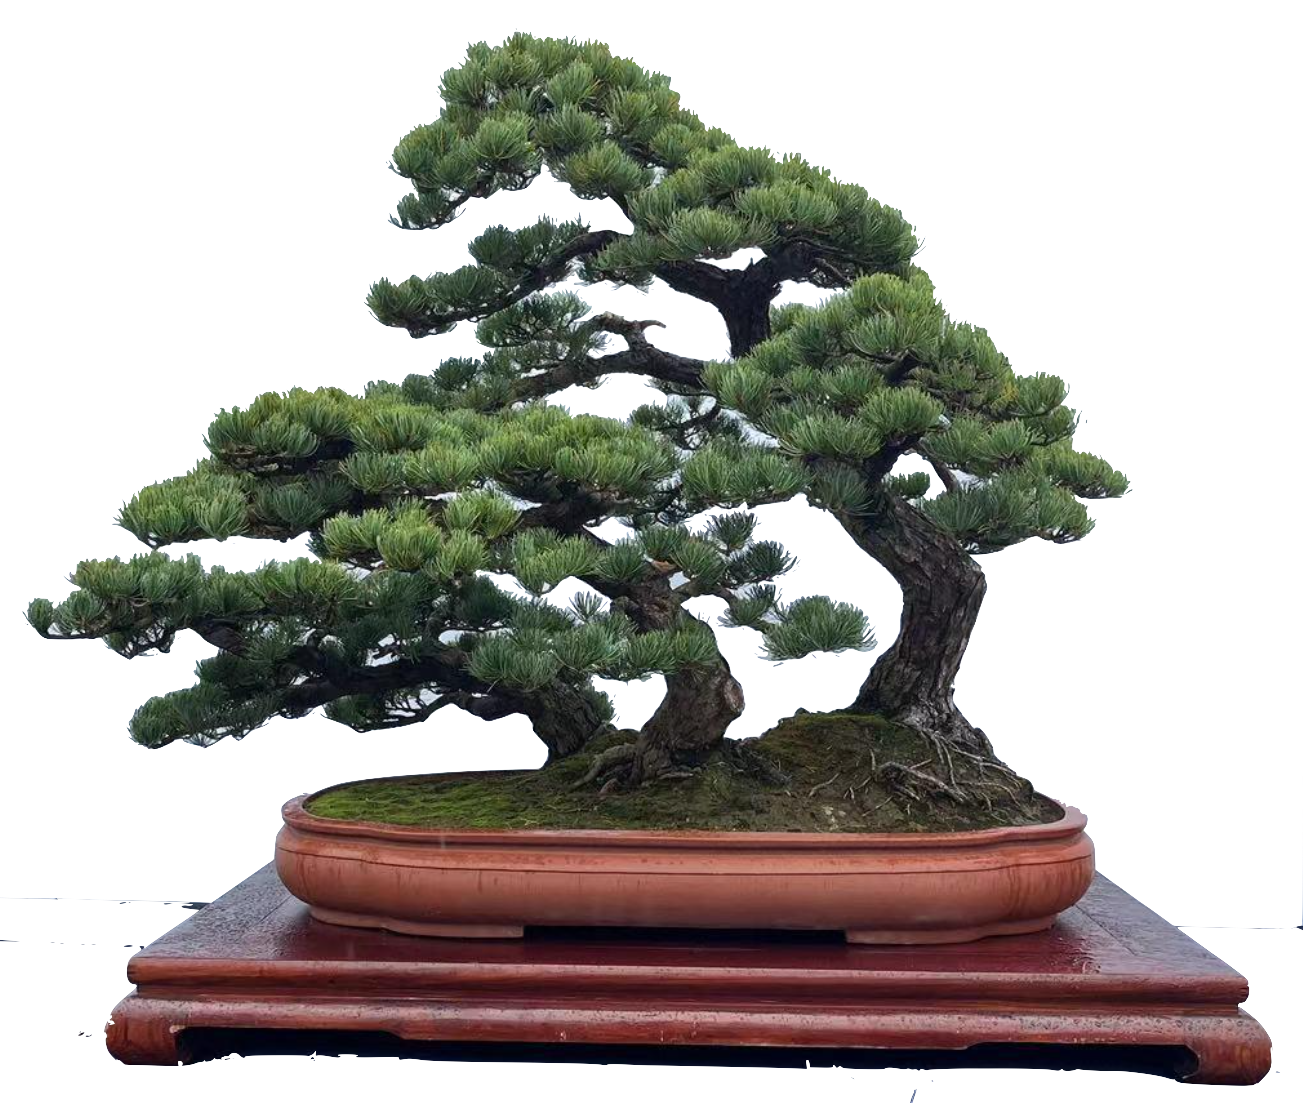
\includegraphics[width=0.95\columnwidth]{res/filler_a.png}
\end{center}

\columnbreak
